\begin{proposition}
  Seja $M$ uma superficie. Então, para cada $k$ existe um único operador linear
  \begin{align*}
    d:\Lambda^{k}(M)&\to\Lambda^{k+1}(M),
  \end{align*}
  chamado o \textbf{operador derivada exterior} que satisfaz as seguintes propriedades
  \begin{enumerate}[i)]
    \item Se $f$ é uma $0$-forma, $df$ é a diferencial de $f$.
    \item Se $w\in\Lambda^{k}(M)$ e $\eta\in\Lambda^{l}(M)$, então
      \begin{align*}
        d(w\wedge\eta)=dw\wedge\eta + (-1)^{k}d\eta\wedge w.
      \end{align*}
    \item $d^{2}=0$.\\
      Em coordenadas locais, se $w=\sum_{J}w_Jdx^{J}$, então
      \begin{align*}
        dw=\sum_{J}dw_J\wedge dx^{J}=\sum_{J}\sum_{i=1}^{n}\frac{\partial w_J}{\partial x^{i}}dx^{i}\wedge dx^{J}.
      \end{align*}
  \end{enumerate}
\end{proposition}
\begin{proof} 
  \begin{center}
    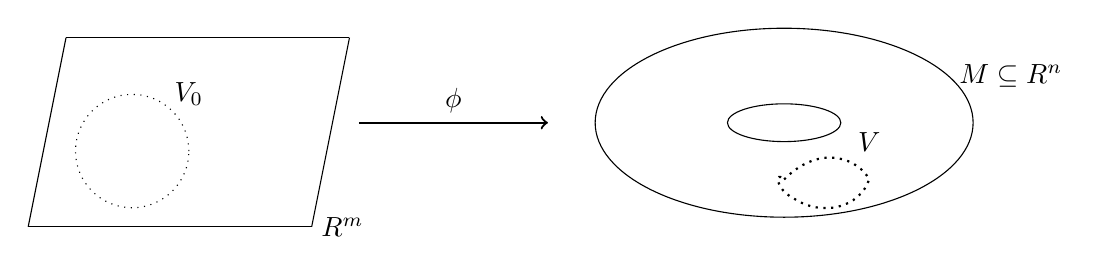
\begin{tikzpicture}[scale=1.2]

% --- Dominio en R^2 ---
\begin{scope}
  \draw[-] (0,0.4) -- (3,0.4) node[right] {$\mathbb{R}^{m}$};
  \draw[-] (0.4,2.4) -- (3.4,2.4);
  \draw[-] (3,0.4) -- (3.4,2.4);
  \draw[-] (0,0.4) -- (0.4,2.4);

  % Abierto (rectángulo)
  \draw[dotted] (1.1,1.2) circle (0.6);

  \node at (1.7,1.8) {$V_0$};
\end{scope}

% Flecha phi
\draw[->, thick] (3.5,1.5) -- (5.5,1.5) node[midway, above] {$\phi$};

% --- Toro (aproximación 2D) ---
\begin{scope}[xshift=8cm]

  % Contorno exterior (elipse grande)
  \draw (0,1.5) ellipse (2 and 1);

  % Agujero interior
  \draw (0,1.5) ellipse (0.6 and 0.2);

\draw[dotted, thick]
  (0,0.9)
  .. controls (0.4,1.3) and (0.8,1.1) ..
  (0.9,0.9)
  .. controls (0.8,0.6) and (0.4,0.5) ..
  (0.1,0.7)
  .. controls (-0.1,0.8) and (-0.1,1) ..
  cycle;

\node at (0.9,1.3) {$V$};
\node at (2.4,2) {$M\subseteq \mathbb{R}^{n}$};
\end{scope}
\end{tikzpicture}

  
  \end{center}
  Dada uma parametrização $(\varphi, V_0)$ para $M$, definimos
  \begin{align*}
    dw=(\varphi^{-1})^{\ast}d\left[ \varphi^{\ast}w \right].
  \end{align*}
  \textbf{Afirmação:}\\
  O operador $d$ de $M$ está bem definido.\\
  De fato, seja $(\psi, U_0)$ uma outra parametrização para vizinhança de $V$ de $M$ com $\varphi(U)\cap\psi(U_0)\neq \emptyset$. Então,
  \begin{align*}
    (\varphi^{-1})^{\ast}d\left[ \varphi^{\ast}w \right]=&(\varphi^{-1}\circ\psi\circ\psi^{-1})^{\ast}d\left[ \varphi^{\ast}w \right]\\
    =&(\psi^{-1})^{\ast}(\varphi^{-1}\circ\psi)^{\ast}d\left[ \varphi^{\ast}w \right]\\
    =&(\psi^{-1})^{\ast}d\left[ (\varphi^{-1}\circ\psi)^{\ast}\varphi^{\ast}w \right]\\
    =&(\psi^{-1})^{\ast}d\left[ (\varphi\circ\varphi^{-1}\circ\psi)^{\ast}w \right]\\
    =&(\psi^{-1})^{\ast}d\left[ \psi^{\ast}w \right].
  \end{align*}
  \textbf{Unicidade:}\\
  \textbf{Afirmação:} Suponha que $w_1$ e $w_2$ são $k$-formas tais que $w_1=w_2$ em um aberto $U$, então $dw_1=dw_2$ em $U$.\\
  De fato, considete $\eta=w_1-w_2$.\\
  Dado $p\in U$, seja $f$ uma função lombada suportada em $U$ (como no exemplo \ref{ex:bumb-function}) 
  \begin{align*}
    f(x)=\begin{cases}
      1, &\text{ se } x\in U_p\subseteq U \text{,} \\
      0, &\text{ se } x\notin U.
    \end{cases}
  \end{align*}
  e $f\in C^{\infty}$ em toda a superfície.\\
  Então temos que $f\eta\equiv 0$, depois temos que
  \begin{align*}
    0=d(f\wedge\eta)=df\wedge\eta+f\wedge d\eta.
  \end{align*}
  Isto é, no ponto $p$, que como $f$ é constante no $U_p$ e $f(p)=1$ temos que 
  \begin{align*}
    0=df_{p}\wedge\eta_{p}+f(p)\wedge d\eta_{p}=d\eta_p.
  \end{align*}
  Para todo $p\in U$, logo temos que $d\eta=0$ em $U$.\\
  Agora, dado $w\in\Lambda^{k}(M)$, escrevala em coordenadas locais em relação a uma carta $(\varphi,U)$ como $w=\sum_{J}w_Jdx^{J}$.\\
  Usando funções lombadas para qualquer $p\in U$ podemos estender as funções $w_J$ é as funções coordenadas $x^{i}$ restritas a uma vizinhança de $p$, a funções diferenciaveis definidas globalmente em $M$
  \begin{align*}
    \tilde{w}_{J}=\sum_{q\in M}f(q)w_J.
  \end{align*}
  Segue-se que
  \begin{align*}
    dw_p=\sum_{J}(dw_J)_{p}\wedge dx^{J}_p.
  \end{align*}
\end{proof}
\begin{proposition}
  Seja $F:M\to N$ uma aplicação diferenciável então
  \begin{align*}
    F^{\ast}(dw)=d(F^{\ast}w).
  \end{align*}
\end{proposition}
\begin{proof} 
  Seja $(\varphi,U)$ uma carta para $M$ e $(\psi,V)$ uma carta para $N$, temos
  \begin{align*}
    F^{\ast}(dw)=&F^{\ast}\left( (\psi^{-1})^{\ast}d\left[ \psi^{\ast}w \right] \right)\\
    =&(\psi^{-1}\circ F)^{\ast}d\left[ \psi^{\ast}w \right]\\
    =&(\psi^{-1}\circ F\circ\varphi\circ\varphi^{-1})^{\ast}d\left[ \psi^{\ast}w \right]\\
    =&(\varphi^{-1})^{\ast}(\psi^{-1}\circ F\circ\varphi)^{\ast}d\left[ \psi^{\ast}w \right]\\
    =&(\varphi^{-1})^{\ast}d\left[ (F\circ\varphi)^{\ast}w \right]\\
    =&d\left[ F^{\ast}w \right].
  \end{align*}
\end{proof}
